\documentclass[11pt,a4paper]{article}
\usepackage[utf8]{inputenc}
\usepackage[margin=1in]{geometry}
\usepackage{tikz}
\usepackage{listings}
\usepackage{xcolor}
\usepackage{hyperref}
\usepackage{tcolorbox}
\usepackage{graphicx}
\usepackage{enumitem}
\usepackage{pmboxdraw}  % For box-drawing characters

\usetikzlibrary{shapes.geometric, arrows, positioning, fit, backgrounds, calc}

% Configure listings to support UTF-8 box-drawing characters
\lstset{
    inputencoding=utf8,
    extendedchars=true,
    literate=
        {├}{{\smash{\raisebox{-0.5ex}{\rule{0.1em}{1.5ex}}}\raisebox{0.5ex}{\rule{0.4em}{0.1em}}}}1
        {│}{{\smash{\raisebox{-0.5ex}{\rule{0.1em}{1.5ex}}}}}1
        {└}{{\smash{\raisebox{0ex}{\rule{0.1em}{0.75ex}}}\raisebox{0.5ex}{\rule{0.4em}{0.1em}}}}1
        {─}{{\raisebox{0.5ex}{\rule{0.6em}{0.1em}}}}1
}

% Define colors
\definecolor{uicolor}{RGB}{102,126,234}
\definecolor{apicolor}{RGB}{118,75,162}
\definecolor{servicecolor}{RGB}{72,187,120}
\definecolor{preprocesscolor}{RGB}{237,137,54}
\definecolor{aicolor}{RGB}{159,122,234}
\definecolor{matchcolor}{RGB}{56,178,172}
\definecolor{annotatecolor}{RGB}{245,158,11}
\definecolor{encodecolor}{RGB}{239,68,68}
\definecolor{responsecolor}{RGB}{139,92,246}
\definecolor{presentcolor}{RGB}{236,72,153}

% TikZ styles
\tikzstyle{block} = [rectangle, draw, fill=blue!20, text width=6em, text centered, rounded corners, minimum height=3em]
\tikzstyle{wideblock} = [rectangle, draw, fill=blue!15, text width=12em, text centered, rounded corners, minimum height=2.5em]
\tikzstyle{arrow} = [thick,->,>=stealth]
\tikzstyle{layer} = [rectangle, draw, fill=gray!10, text width=15cm, text centered, minimum height=1.5cm, rounded corners]

\title{\textbf{ThriftAssist System Block Diagram}}
\author{System Architecture Documentation}
\date{\today}

\begin{document}

\maketitle

\section*{System Architecture Overview}

ThriftAssist is a comprehensive OCR-based phrase detection system that identifies specific text phrases in images using Google Cloud Vision API, applies intelligent multi-strategy matching, annotates results visually, and presents them through a responsive web interface.

\section{High-Level Architecture}

\begin{center}
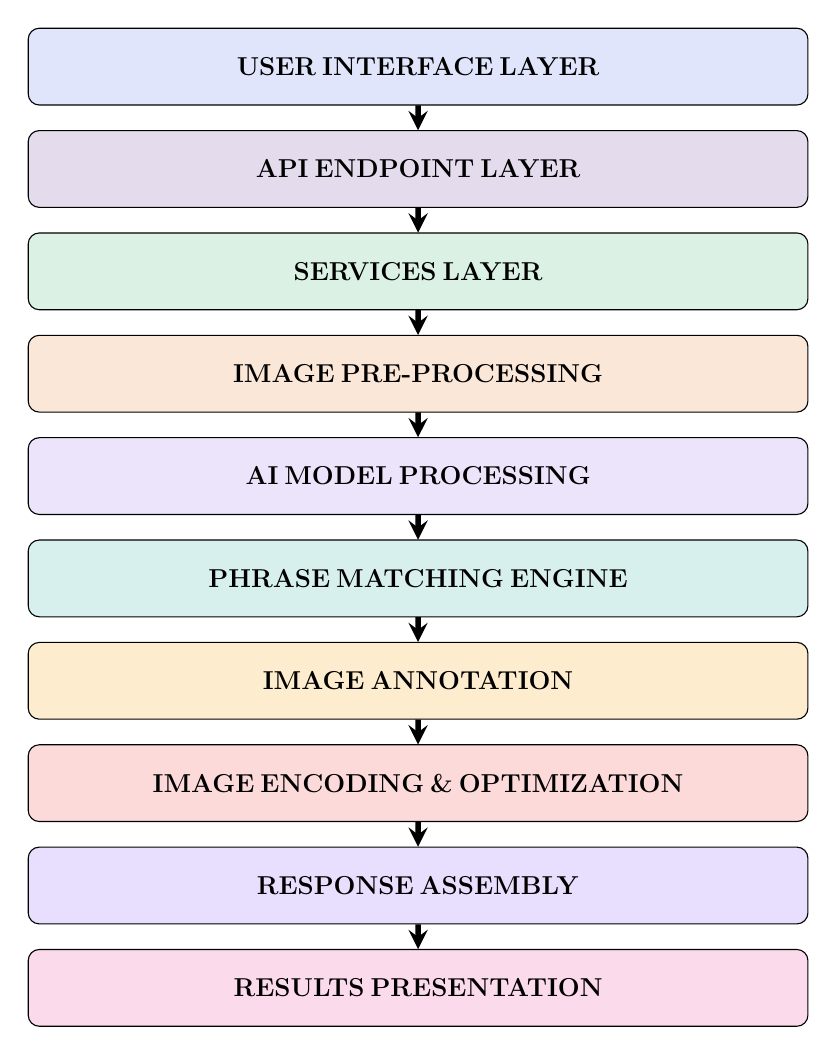
\begin{tikzpicture}[node distance=1.2cm, scale=0.65, transform shape]

% Layer boxes
\node[layer, fill=uicolor!20] (ui) at (0,0) {\Large\textbf{USER INTERFACE LAYER}};
\node[layer, fill=apicolor!20] (api) at (0,-2) {\Large\textbf{API ENDPOINT LAYER}};
\node[layer, fill=servicecolor!20] (service) at (0,-4) {\Large\textbf{SERVICES LAYER}};
\node[layer, fill=preprocesscolor!20] (preprocess) at (0,-6) {\Large\textbf{IMAGE PRE-PROCESSING}};
\node[layer, fill=aicolor!20] (ai) at (0,-8) {\Large\textbf{AI MODEL PROCESSING}};
\node[layer, fill=matchcolor!20] (match) at (0,-10) {\Large\textbf{PHRASE MATCHING ENGINE}};
\node[layer, fill=annotatecolor!20] (annotate) at (0,-12) {\Large\textbf{IMAGE ANNOTATION}};
\node[layer, fill=encodecolor!20] (encode) at (0,-14) {\Large\textbf{IMAGE ENCODING \& OPTIMIZATION}};
\node[layer, fill=responsecolor!20] (response) at (0,-16) {\Large\textbf{RESPONSE ASSEMBLY}};
\node[layer, fill=presentcolor!20] (present) at (0,-18) {\Large\textbf{RESULTS PRESENTATION}};

% Arrows between layers
\draw[arrow, line width=2pt] (ui) -- (api);
\draw[arrow, line width=2pt] (api) -- (service);
\draw[arrow, line width=2pt] (service) -- (preprocess);
\draw[arrow, line width=2pt] (preprocess) -- (ai);
\draw[arrow, line width=2pt] (ai) -- (match);
\draw[arrow, line width=2pt] (match) -- (annotate);
\draw[arrow, line width=2pt] (annotate) -- (encode);
\draw[arrow, line width=2pt] (encode) -- (response);
\draw[arrow, line width=2pt] (response) -- (present);

\end{tikzpicture}
\end{center}

\newpage

\section{Component Details}

\subsection{User Interface Layer}
\textbf{Location:} \texttt{public/web\_app.html}

\begin{tcolorbox}[colback=uicolor!10, colframe=uicolor!80, title=UI Components]
\begin{itemize}[leftmargin=*]
    \item \textbf{Input Form}
    \begin{itemize}
        \item File upload (single/batch mode)
        \item Search phrases input
        \item Threshold slider (50-100\%)
        \item Text scale control
    \end{itemize}
    
    \item \textbf{Gallery View}
    \begin{itemize}
        \item Thumbnail preview
        \item Multi-select capability
        \item Image selection controls
        \item Add/remove images
    \end{itemize}
    
    \item \textbf{Results Display}
    \begin{itemize}
        \item Match summary statistics
        \item Confidence metrics
        \item Explainability panels
        \item Annotated image with zoom/pan
    \end{itemize}
\end{itemize}
\end{tcolorbox}

\newpage    

\subsection{API Endpoint Layer}
\textbf{Location:} \texttt{backend/api/routes/ocr.py}

\begin{tcolorbox}[colback=apicolor!10, colframe=apicolor!80, title=/upload-and-detect Endpoint]
\textbf{Request Processing Pipeline:}
\begin{enumerate}[leftmargin=*]
    \item Validate input (file type, size, parameters)
    \item Generate cache key (MD5 hash of image + text\_scale)
    \item Check cache for existing result
    \begin{itemize}
        \item If cache hit → Return cached result immediately
        \item If cache miss → Continue processing
    \end{itemize}
    \item Save temporary image file
    \item Resize image if width $>$ max\_image\_width
    \item Invoke OCR processing
    \item Format match results
    \item Encode annotated image to base64
    \item Cache result for future requests
    \item Return JSON response
\end{enumerate}
\end{tcolorbox}

\subsection{Services Layer}
\textbf{Location:} \texttt{backend/services/}

\begin{tcolorbox}[colback=servicecolor!10, colframe=servicecolor!80, title=Service Components]
\begin{description}[leftmargin=3cm, style=nextline]
    \item[Image Service] Validates image format, decodes base64, saves temporary files, manages cleanup
    
    \item[Cache Service] Implements MD5 hashing, LRU cache with TTL, automatic eviction, cache hit/miss tracking
    
    \item[OCR Service] Orchestrates detection pipeline, formats results for API, measures processing time, coordinates with Vision API
\end{description}
\end{tcolorbox}

\newpage

\subsection{Image Pre-Processing}
\textbf{Location:} OpenCV/PIL Pipeline

\begin{tcolorbox}[colback=preprocesscolor!10, colframe=preprocesscolor!80, title=Pre-Processing Steps]
\begin{enumerate}[leftmargin=*]
    \item Load image using \texttt{cv2.imread()}
    \item Check dimensions against \texttt{max\_image\_width}
    \item Resize if necessary (maintaining aspect ratio)
    \item Optimize for display performance
    \item Save as temporary file for Vision API
\end{enumerate}
\end{tcolorbox}

\subsection{AI Model Processing}
\textbf{Location:} \texttt{vision/detector.py}

\begin{tcolorbox}[colback=aicolor!10, colframe=aicolor!80, title=Google Cloud Vision API Integration]
\textbf{VisionPhraseDetector.detect() Process:}
\begin{enumerate}[leftmargin=*]
    \item \textbf{Call Google Vision API}
    \begin{itemize}
        \item Execute \texttt{document\_text\_detection()}
        \item Extract full text annotations
        \item Retrieve bounding boxes and vertices
    \end{itemize}
    
    \item \textbf{Parse Text Lines}
    \begin{itemize}
        \item Extract text content from annotations
        \item Calculate Y-position (vertical location)
        \item Determine rotation angle
        \item Store bounding box coordinates
    \end{itemize}
    
    \item \textbf{Build Text Structure}
    \begin{itemize}
        \item Sort lines by Y-position
        \item Group multi-line text blocks
        \item Preserve spatial relationships
    \end{itemize}
\end{enumerate}
\end{tcolorbox}

\newpage

\subsection{Phrase Matching Engine}
\textbf{Location:} \texttt{vision/matcher.py}

\begin{tcolorbox}[colback=matchcolor!10, colframe=matchcolor!80, title=PhraseMatcher.find\_matches()]
\textbf{Multi-Strategy Matching:}

\begin{enumerate}[label=\Alph*., leftmargin=*]
    \item \textbf{EXACT MATCHING}
    \begin{itemize}
        \item Case-insensitive comparison
        \item Direct string match
        \item 100\% confidence score
    \end{itemize}
    
    \item \textbf{FUZZY MATCHING (RapidFuzz)}
    \begin{itemize}
        \item Levenshtein distance calculation
        \item Partial ratio scoring
        \item Token-based matching
        \item Similarity score (0-100)
    \end{itemize}
    
    \item \textbf{MULTI-LINE SPANNING}
    \begin{itemize}
        \item Combine adjacent text lines
        \item Match phrases split across lines
        \item Window-based search (2-3 lines)
    \end{itemize}
    
    \item \textbf{UPSIDE-DOWN DETECTION}
    \begin{itemize}
        \item Check rotation angles ($\pm$180°)
        \item Reverse text comparison
        \item Match inverted text
    \end{itemize}
    
    \item \textbf{THRESHOLD FILTERING}
    \begin{itemize}
        \item Apply user-defined threshold (50-100\%)
        \item Filter low-confidence matches
        \item Rank by similarity score
    \end{itemize}
    
    \item \textbf{DEDUPLICATION}
    \begin{itemize}
        \item Remove duplicate matches
        \item Merge overlapping bounding boxes
        \item Keep highest-confidence match
    \end{itemize}
\end{enumerate}
\end{tcolorbox}

\newpage

\subsection{Image Annotation}
\textbf{Location:} \texttt{vision/detector.py + OpenCV}

\begin{tcolorbox}[colback=annotatecolor!10, colframe=annotatecolor!80, title=Annotation Process]
\begin{enumerate}[leftmargin=*]
    \item \textbf{Draw Bounding Boxes}
    \begin{itemize}
        \item Green rectangles around matches
        \item Line thickness based on confidence
        \item Color intensity varies by score
    \end{itemize}
    
    \item \textbf{Add Text Labels}
    \begin{itemize}
        \item Display match phrase text
        \item Show confidence percentage
        \item Font size scaled by \texttt{text\_scale} parameter
        \item Positioned above/below bounding box
        \item Mobile boost: 4$\times$ text scale for mobile devices
    \end{itemize}
    
    \item \textbf{Handle Overlaps}
    \begin{itemize}
        \item Adjust label positions to avoid overlap
        \item Layer annotations by confidence
    \end{itemize}
    
    \item \textbf{Maintain Image Quality}
    \begin{itemize}
        \item Preserve original aspect ratio
        \item Anti-aliasing for smooth rendering
    \end{itemize}
\end{enumerate}
\end{tcolorbox}

\newpage

\subsection{Image Encoding \& Optimization}
\textbf{Location:} \texttt{backend/utils/image\_utils.py}

\begin{tcolorbox}[colback=encodecolor!10, colframe=encodecolor!80, title=Encoding Pipeline]
\begin{enumerate}[leftmargin=*]
    \item \textbf{Convert to PIL Image}
    \begin{itemize}
        \item OpenCV BGR $\rightarrow$ RGB conversion
        \item Maintain numpy array structure
    \end{itemize}
    
    \item \textbf{Calculate Optimal JPEG Quality}
    \begin{itemize}
        \item Based on image dimensions
        \item Larger images: lower quality (60-75)
        \item Smaller images: higher quality (85-95)
        \item Balance file size vs visual quality
    \end{itemize}
    
    \item \textbf{Encode to Base64}
    \begin{itemize}
        \item JPEG compression with calculated quality
        \item Optimization enabled
        \item Base64 encoding for JSON transport
    \end{itemize}
    
    \item \textbf{Memory Management}
    \begin{itemize}
        \item Immediate cleanup of temporary objects
        \item Garbage collection after encoding
    \end{itemize}
\end{enumerate}
\end{tcolorbox}

\newpage
\subsection{Response Assembly}
\textbf{Location:} \texttt{backend/api/routes/ocr.py}

\begin{tcolorbox}[colback=responsecolor!10, colframe=responsecolor!80, title=JSON Response Structure]
\begin{lstlisting}[basicstyle=\small\ttfamily, breaklines=true, escapechar=!]
{
  "success": true,
  "total_matches": !$\langle$!count!$\rangle$!,
  "matches": {
    "phrase1": [
      {
        "text": "matched text",
        "score": 95.5,
        "match_type": "exact|fuzzy|spanning|upside_down",
        "angle": 0,
        "bounding_box": [[x1,y1], [x2,y2], ...],
        "explanation": {
          "confidence_level": "Very High|High|Medium|Low",
          "reasoning": ["reason1", "reason2"],
          "recommendation": "explanation text"
        }
      }
    ]
  },
  "processing_time_ms": 1234.5,
  "image_dimensions": [width, height],
  "annotated_image_base64": "base64_encoded_jpeg",
  "cached": false
}
\end{lstlisting}
\end{tcolorbox}

\newpage

\subsection{Results Presentation (UI)}
\textbf{Location:} \texttt{public/web\_app.html}

\begin{tcolorbox}[colback=presentcolor!10, colframe=presentcolor!80, title=UI Presentation Components]
\begin{description}[leftmargin=3cm, style=nextline]
    \item[Results Summary] Display total matches, processing time, average confidence, image dimensions
    
    \item[Match Details] Collapsible cards grouped by search phrase with:
    \begin{itemize}
        \item Individual match items
        \item Matched text preview
        \item Confidence badges (Very High, High, Medium, Low)
        \item Similarity score percentage
        \item Rotation angle indicator
    \end{itemize}
    
    \item[Explainability] ``Why?'' button reveals:
    \begin{itemize}
        \item Confidence level explanation
        \item Reasoning factors list
        \item Match type description
        \item User recommendations
    \end{itemize}
    
    \item[Annotated Image Display] Features:
    \begin{itemize}
        \item Base64 decode $\rightarrow$ data URL
        \item Responsive sizing (mobile/tablet/desktop)
        \item Aspect ratio preservation
        \item Zoom \& pan controls (Panzoom.js)
        \item Touch gesture support
        \item Device-specific optimizations
    \end{itemize}
    
    \item[Batch Mode Results] For multiple images:
    \begin{itemize}
        \item Batch summary (total images, success count)
        \item Individual image result cards
        \item Per-image annotated display
        \item Click to enlarge (modal view)
    \end{itemize}
\end{description}
\end{tcolorbox}

\section{Data Flow Diagrams}

\subsection{Single Image Processing Flow}

\begin{center}
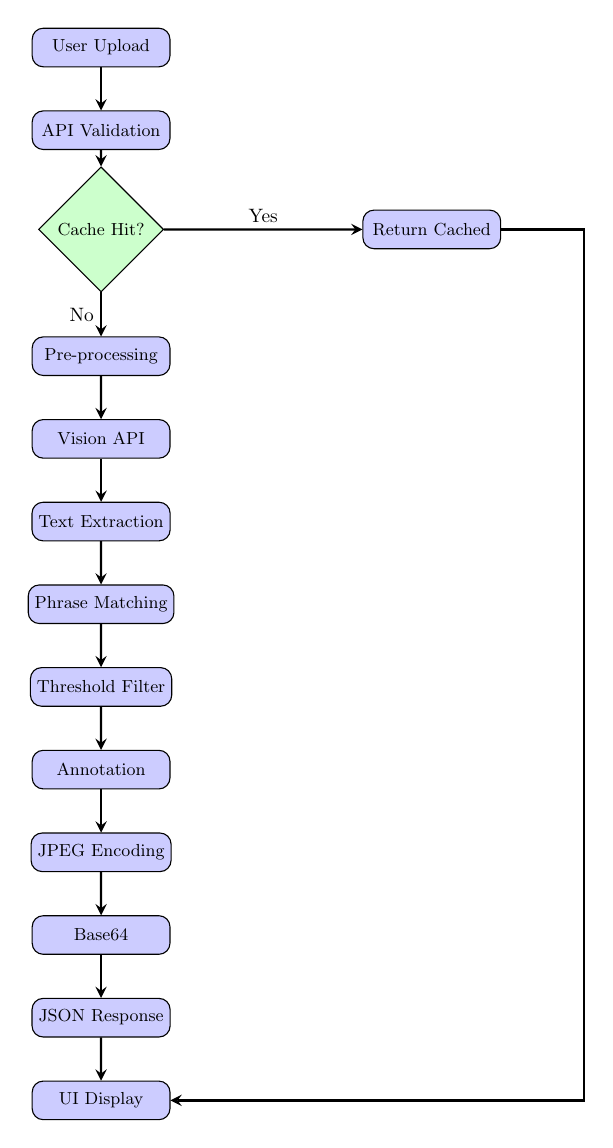
\begin{tikzpicture}[node distance=1.5cm, scale=0.7, transform shape]
\tikzstyle{process} = [rectangle, rounded corners, minimum width=2.5cm, minimum height=0.7cm, text centered, draw=black, fill=blue!20, font=\small]
\tikzstyle{decision} = [diamond, minimum width=2cm, minimum height=0.7cm, text centered, draw=black, fill=green!20, font=\small]
\tikzstyle{arrow} = [thick,->,>=stealth]

\node (upload) [process] {User Upload};
\node (validate) [process, below of=upload] {API Validation};
\node (cache) [decision, below of=validate, yshift=-0.3cm] {Cache Hit?};
\node (cached) [process, right of=cache, xshift=4.5cm] {Return Cached};
\node (preprocess) [process, below of=cache, yshift=-0.8cm] {Pre-processing};
\node (vision) [process, below of=preprocess] {Vision API};
\node (extract) [process, below of=vision] {Text Extraction};
\node (match) [process, below of=extract] {Phrase Matching};
\node (filter) [process, below of=match] {Threshold Filter};
\node (annotate) [process, below of=filter] {Annotation};
\node (encode) [process, below of=annotate] {JPEG Encoding};
\node (base64) [process, below of=encode] {Base64};
\node (json) [process, below of=base64] {JSON Response};
\node (display) [process, below of=json] {UI Display};

\draw [arrow] (upload) -- (validate);
\draw [arrow] (validate) -- (cache);
\draw [arrow] (cache) -- node[anchor=east] {No} (preprocess);
\draw [arrow] (cache) -- node[anchor=south] {Yes} (cached);
\draw [arrow] (cached.east) -- ++(1.5,0) |- (display.east);
\draw [arrow] (preprocess) -- (vision);
\draw [arrow] (vision) -- (extract);
\draw [arrow] (extract) -- (match);
\draw [arrow] (match) -- (filter);
\draw [arrow] (filter) -- (annotate);
\draw [arrow] (annotate) -- (encode);
\draw [arrow] (encode) -- (base64);
\draw [arrow] (base64) -- (json);
\draw [arrow] (json) -- (display);

\end{tikzpicture}
\end{center}

\subsection{Batch Processing Flow}

\begin{center}
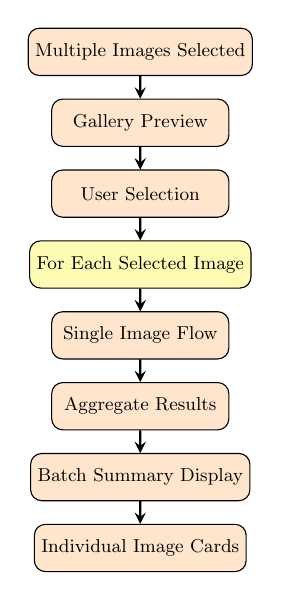
\begin{tikzpicture}[node distance=1.2cm, scale=0.75, transform shape]
\tikzstyle{process} = [rectangle, rounded corners, minimum width=3cm, minimum height=0.8cm, text centered, draw=black, fill=orange!20, font=\small]
\tikzstyle{loop} = [rectangle, rounded corners, minimum width=3cm, minimum height=0.8cm, text centered, draw=black, fill=yellow!30, font=\small]
\tikzstyle{arrow} = [thick,->,>=stealth]

\node (select) [process] {Multiple Images Selected};
\node (gallery) [process, below of=select] {Gallery Preview};
\node (userselect) [process, below of=gallery] {User Selection};
\node (loop) [loop, below of=userselect] {For Each Selected Image};
\node (single) [process, below of=loop] {Single Image Flow};
\node (aggregate) [process, below of=single] {Aggregate Results};
\node (summary) [process, below of=aggregate] {Batch Summary Display};
\node (cards) [process, below of=summary] {Individual Image Cards};

\draw [arrow] (select) -- (gallery);
\draw [arrow] (gallery) -- (userselect);
\draw [arrow] (userselect) -- (loop);
\draw [arrow] (loop) -- (single);
\draw [arrow] (single) -- (aggregate);
\draw [arrow] (aggregate) -- (summary);
\draw [arrow] (summary) -- (cards);

\end{tikzpicture}
\end{center}

\section{Key Performance Features}

\begin{tcolorbox}[colback=gray!5, colframe=gray!60, title=Performance Optimizations]
\begin{enumerate}[leftmargin=*]
    \item \textbf{Caching Layer}
    \begin{itemize}
        \item MD5-based LRU cache with TTL
        \item Avoids redundant OCR processing
        \item Significant performance improvement for repeated queries
    \end{itemize}
    
    \item \textbf{Image Optimization}
    \begin{itemize}
        \item Automatic resizing for large images
        \item Dynamic JPEG quality adjustment
        \item Optimal balance between quality and transfer size
    \end{itemize}
    
    \item \textbf{Memory Management}
    \begin{itemize}
        \item Aggressive cleanup throughout pipeline
        \item Explicit garbage collection
        \item Prevents memory leaks in long-running processes
    \end{itemize}
    
    \item \textbf{Responsive Design}
    \begin{itemize}
        \item Device-specific rendering
        \item Mobile/tablet/desktop optimizations
        \item Touch gesture support
    \end{itemize}
    
    \item \textbf{Batch Processing}
    \begin{itemize}
        \item Sequential processing with progress tracking
        \item Individual error handling per image
        \item Parallel-ready architecture
    \end{itemize}
    
    \item \textbf{Explainability}
    \begin{itemize}
        \item Detailed reasoning for each match
        \item Confidence metrics and recommendations
        \item Transparent AI decision-making
    \end{itemize}
\end{enumerate}
\end{tcolorbox}

\newpage

\section{Technology Stack}

\begin{table}[h]
\centering
\begin{tabular}{|l|l|}
\hline
\textbf{Component} & \textbf{Technology} \\ \hline
Frontend & Vanilla JavaScript, HTML5, CSS3, Panzoom.js \\ \hline
Backend & FastAPI (Python), Uvicorn ASGI server \\ \hline
AI/ML & Google Cloud Vision API, RapidFuzz \\ \hline
Image Processing & OpenCV (cv2), PIL/Pillow \\ \hline
Caching & In-memory LRU cache (OrderedDict) \\ \hline
Data Transport & Base64-encoded JPEG in JSON \\ \hline
\end{tabular}
\caption{Technology Stack Components}
\end{table}

\section{File Structure Reference}

\begin{lstlisting}[basicstyle=\small\ttfamily, breaklines=true]
thrift_assist/
├── public/
│   └── web_app.html              # Frontend UI
├── backend/
│   ├── api/
│   │   ├── main.py               # FastAPI application
│   │   └── routes/
│   │       └── ocr.py            # /upload-and-detect endpoint
│   ├── services/
│   │   ├── image_service.py      # Image validation & I/O
│   │   ├── cache_service.py      # LRU caching
│   │   └── ocr_service.py        # OCR orchestration
│   ├── utils/
│   │   └── image_utils.py        # JPEG quality calculation
│   └── core/
│       └── config.py             # Configuration settings
├── vision/
│   ├── detector.py               # Vision API integration
│   └── matcher.py                # Phrase matching engine
└── utils/
    └── text_utils.py             # Text normalization
\end{lstlisting}

\end{document}
